% Supporting Information for "Minimum-Seismicity Injection Design Is Convex, and the Value of Design Is Set by Two Numbers" (GRL)
\documentclass[11pt]{article}
\usepackage[a4paper,margin=25mm]{geometry}
\usepackage{amsmath,amssymb,graphicx,url,booktabs}
\title{Supporting Information for ``Minimum-Seismicity Injection Design Is Convex, and the Value of Design Is Set by Two Numbers''}
\author{[Authors]}
\date{Geophysical Research Letters --- draft v0.5}
\begin{document}
\maketitle
\noindent\textbf{Contents:} Text S1 ($\theta$-law, three-arc optimum), Text S2 (synthetic set-up and verification), Text S3 (pre-registered
field tests), Text S4 (simulator design and coupled case), Table S1, Figures S1--S2.

\section*{Text S1. Three-arc optimum and the $\theta$-law}
Time is normalised by $T_{inj}$ and the volume to one. The stress obeys $\theta\dot s=u-s$, $s(0)=0$, with $u\in[0,u_{\max}]$,
$\int_0^1u\,\mathrm{d}t=1$; the tail decays freely. Per unit background rate, $J=\int_0^\infty(e^{\Pi s/s_c}-1)\mathrm{d}t$ with
$s_c=1-e^{-1/\theta}$. The Hamiltonian is linear in $u$; on a singular arc $\partial H/\partial u\equiv0$ implies $\dot\lambda=0$ and hence a
constant stress $s^*$ with $u=s^*$. The optimum is: charging at $u_{\max}$ for $t_r=\theta\ln(u_{\max}/(u_{\max}-s^*))$, plateau, and a
maximum-rate burst before shut-in (for $u_{\max}=10$, $\theta\gtrsim0.1$ a coasting arc can precede it). Constant rate gives
$J_c=(e^\Pi-1)-\theta e^\Pi\,\mathrm{Ein}(\Pi)+\theta[\mathrm{Ei}(\Pi)-\gamma-\ln\Pi]$ for $\theta\ll1$, with
$\mathrm{Ein}(x)=\int_0^x(1-e^{-y})/y\,\mathrm{d}y$. To first order, $G=1-J^*/J_c=\theta\kappa_2(\Pi,u_{\max})+O(\theta^2)$ with
$\kappa=e^\Pi[\Pi m+R-\mathrm{Ein}(\Pi)]/(e^\Pi-1)$, $m=(u_{\max}-1)\ln(u_{\max}/(u_{\max}-1))$, $R$ the start-up layer term.
A direct discretised optimal-control solution agrees with the closed form to $\sim10^{-5}$; the first-order term is accurate to +5--8\% up to
$\theta=0.1$ (script \texttt{research/exp/h1f\_theta\_law.py}).

\section*{Text S2. Synthetic set-up and verification}
3-D point-source diffusion with exact erfc step responses; $k=10^{-14}$~m$^2$, $\mu=10^{-3}$~Pa\,s, diffusivity 0.1~m$^2$/s, friction 0.6,
$A\bar\sigma=0.05$~MPa, $t_a=100$~yr, patch at 300~m, 8640~m$^3$ in 10~days, rate bound three times the mean, 100 control intervals,
counting to five injection times. Optimisation: SLSQP with the analytic adjoint gradient (softmax weights). Verification: ODE vs integral
form to $10^{-5}$; 2000 midpoint convexity tests (Figure S1a); gradient vs finite differences; multistart; KKT residual; dose invariance to
0.1\%. Excess events (shut-in / total): constant 16.36 / 38.83, step-up 12.21 / 40.49, taper 20.81 / 40.16, optimum 14.14 / 37.01.

\section*{Text S3. Pre-registered field tests}
Pipeline: kernel (multi-exponential, rate $\to$ wellhead pressure), Dieterich with threshold $P^*$ and diffusion time $\tau_d$, counts above
$M_c$. Plans were written before any fit (\texttt{research/CYCLE3\_PLAN.md}, \texttt{CYCLE6\_PLAN.md}). These are internal plan files, not deposited with an external registry, so their dates are not independently time-stamped; they are archived unchanged with the code.
\begin{center}\small
\begin{tabular}{llll}\toprule
Test & Criterion & 2018 & 2020 \\\midrule
E1 kernel hold-out & RMSE $\le$10\% of range & PASS (6.1\%) & WEAK (11.4\%) \\
E2 Dieterich fit & corr $\ge$0.98, tail $\pm$30\% & WEAK (tail +50\%) & PASS (0.998, +8\%) \\
E3 temporal hold-out & end $\pm$30\% & FAIL (+29\% shut-in) & FAIL (degenerate $P^*$) \\
E4 gain optimum vs constant & 2020: $\le$3\% predicted & 1.6\% & \textbf{9.1\% (refuted)} \\
E8 $\theta$-scan peak & in [0.05, 1] & 0.26 & \textbf{0.26 (confirmed)} \\
E9 transfer of 2018 parameters & corr $\ge$0.95 & --- & PASS (0.985) \\
E6 design from hold-out & keeps gain & PASS (70\%) & FAIL (2.9$\times$) \\\bottomrule
\end{tabular}\end{center}
2020 values: $V=2884$~m$^3$, shut-in 387.3~h, 6121 events ($M_c=-1.45$, $b=1.39$), $P^*=72.9$~bar, $\tau_d=10.0$~h, $\Pi=3.43$;
$\theta$-scan gains 2.4 / 7.6 / 14.0 / 11.5 / 5.8\% at $\theta=0.026$ / 0.078 / 0.26 / 0.77 / 2.58. With pauses imposed: constant 3816,
optimum 2747 events.

\section*{Text S4. Simulator design and coupled case}
Table S1: designed vs constant rate on a heterogeneous $41\times41$ case.
\begin{center}\small\begin{tabular}{lll}\toprule & Constant rate & Designed \\\midrule
Expected events, design model & 127.9 & 100.2 \\ Expected events, simulated & 143.8 & 117.8 ($-18.0$\%) \\
Model error & 17.8\% (first pass) & 0.15\% (after one correction) \\\bottomrule\end{tabular}\end{center}
Coupled case (\texttt{examples/FAULT\_INJECTION.DATA}): $30\times20\times5$ cells of $50\times50\times10$~m at 1975~m, fault with 100 faces
(MULTFLT 0.05) 150~m from a water injector (800~sm$^3$/d, 280~bar cap, shut-in at 500~d); $S_v$ gradient 0.24~bar/m,
$S_{hmin}/S_v=0.65$, $S_{Hmax}/S_v=1.10$ at 60$^\circ$, stress path 0.5, $\mu=0.6$, $t_a=100$~yr, $r_0=5$~km$^{-2}$yr$^{-1}$, $b=1$;
two-way factor 20. Maximum $\Delta$CFS 14.6 (two-way) vs 11.2~bar; 483 sampled events, largest $M_w$ 2.27 (Figure S2). A rate-and-state trace
($a=0.010$, $b=0.015$, $D_c=1$~mm) produced no dynamic rupture ($h^*=920$~m exceeds the 1-km trace).

\begin{figure}[p]\centering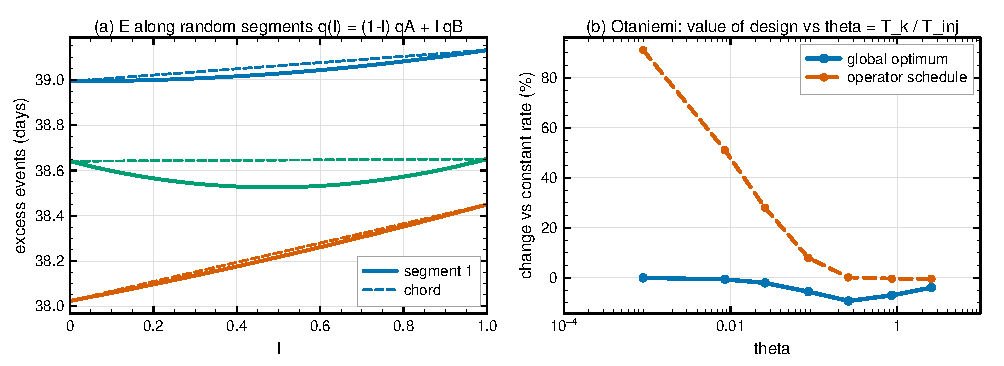
\includegraphics[width=\textwidth]{figs/FigureS1.pdf}
\caption*{\textbf{Figure S1.} (a) Expected events along segments between random feasible schedules lie on or below the chord. (b) Otaniemi 2018:
change relative to constant rate of the optimum and of the operator schedule versus $\theta$.}\end{figure}
\begin{figure}[p]\centering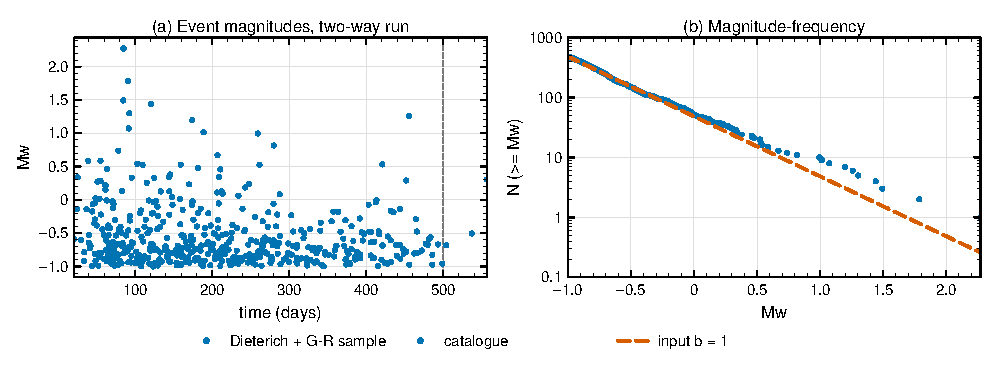
\includegraphics[width=\textwidth]{figs/FigureS2.pdf}
\caption*{\textbf{Figure S2.} Stochastic catalogue of the two-way run: magnitudes versus time and magnitude--frequency distribution (input $b=1$).}\end{figure}
\end{document}
